\documentclass{article}
\usepackage{tikz}
\usepackage{hyperref}
\usepackage{amsmath}
\usepackage{mathtools}
\usepackage{float}
\usepackage{xcolor}
\usepackage[a4paper]{geometry}
\usepackage[textsize=small,textwidth=100]{todonotes}

\usetikzlibrary{positioning,arrows,backgrounds}
\usepgflibrary{shapes.geometric}

\tikzset{%
vertex/.style={draw,fill,circle,minimum size=5pt,inner sep=1pt},
hyperedge/.style={draw,rectangle},
tentacle/.style={pos=0.2,auto,font=\tiny,minimum size=1pt,inner sep=1pt},
flowcond/.style={diamond,minimum size=40pt,draw},
tinylabel/.style={font=\tiny,inner sep=1pt,right=0mm of #1},
every label/.style={font=\tiny,inner sep=1pt,label position=right},
blank/.style={inner sep=0,minimum size=0}
}

\newcommand{\code}[1]{\texttt{#1}}

\begin{document}
\title{Generating Random Graphs with Graph Grammars}
\author{Jake Coxon}
\maketitle

\tableofcontents

\section{Introduction}
Introduction should go here

\section{Literature Review}

\subsection{Graphs}
  \begin{figure}
  \centering
  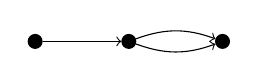
\begin{tikzpicture}
    \node[vertex] (a)    {};
    \node[vertex] (b) [right=of a]  {};
    \node[vertex] (c) [right=of b]  {};
    \path[->] (a) edge (b)
              (b) edge [bend left=20] (c) 
                  edge [bend right=20] (c);
  \end{tikzpicture}
  \caption{A directed multigraph}
\end{figure}

  A graph is a finite set of points known as vertices that are interconnected by a set of lines (edges). Edges connect exactly two vertices that shows a relation.

  A label alphabet $L = \langle L_v, L_e \rangle$ consists of a set $L_v$ of node labels and a set $L_e$ of edge labels.

  A graph over $L$ is a system $G = \langle V_G, E_G, s_G, t_G, l_G, m_G \rangle$ where $V_G$ and $E_G$ are finite sets of vertices and edges respectively. $s_G, t_G : E_G \to V_G$ are functions assigning a source and a target to each edge. $l_G : V_G \to L_V$ and $m_G : E_G \to L_E$ are functions assigning a label to each node and edge\cite{Detlef1}.

  Different types of graphs exist pertaining to different problems. Graph edges can be weighted and/or directed and vertices can be labelled. Graphs can allow edges to be looped where both endpoints point to the same vertex. Multi-graphs are graphs where multiple edges can exist between a pair a vertices.

\subsection{Hypergraphs}
  \begin{figure}
  \centering
  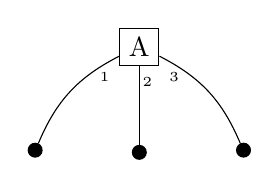
\begin{tikzpicture}

    \node[hyperedge] (hyp)    {A};
    \node[vertex] (a) [below left=of hyp] {};
    \node[vertex] (b) [below=of hyp]  {};
    \node[vertex] (c) [below right=of hyp] {};


    \path[-] (hyp) edge [bend right=20] node[tentacle]{$1$} (a)
                   edge [-] node[tentacle]{$2$} (b)
                   edge [bend left=20] node[tentacle,auto=right]{$3$} (c);
  \end{tikzpicture}
  \caption{A hypergraph with a hyperedge labeled $A$}
\end{figure}

  A generalised version of graphs are hypergraphs. Within a hypergraph, a hyperedge is similar to an edge except it is connected to any number of vertices. The connections between a hyperedge and a vertex is known as `tentacles' and the number of the tentacles a hyperedge has is known as its type. A graph is a specialised version of a hypergraph where all hyperedges has type of $2$.

  An alphabet $C$ is a fixed set containing labels. A hypergraph over $C$ is a system $F = \langle V_F, E_F, att_F, lbl_F \rangle$ where $V_F$ and $E_F$ are finite sets of vertices and edges the same as graphs. $att_F : E_F \to V_F*$ is a mapping assigning a sequence of `attachment nodes' to each edge $e \in E_F$, $att_F(e, i)$ can be written to denote the $i$th attachment node of $e$. $lbl_F$ is a mapping that labels hyperedges. 

  The $type(E)$ of an edge is the number of vertices that a hyperedge attaches to. A tentacle is an object used to describe the attachment of a hyperedge to a vertex.

  Hyperedge can be drawn as a regular edge if its type is 2 and it has no label.

  %\todo{C???}

  \begin{figure}[!h]
  \centering
  \begin{tikzpicture}
    \node[] (a)    {};
    \node[flowcond] (cond) [below=of a]  {};
    \node[] (b) [below left=of cond]  {};
    \node[] (c) [below right=of cond] {};

    \path[<-] (cond) edge (a);
    \draw[->] (cond) -| (b);
    \draw[->] (cond) -| (c);
  \end{tikzpicture}
  \caption{Hyperedges can be used to model flowcharts}
\end{figure}

\subsection{Random Graph Generation}
  Random graph generators are systems to generate a single or set of graphs based on some non-deterministic rules. This can be used as test data for programs for testing speed and memory. It can also be used for verifying whether a property is true for a range of graphs in a range or seeing how \emph{often} a property is true for a range of graphs.

  There are two methods for random graph generation described in \cite{Skiena}:

  Random Edge Generation---Every pair of vertices is listed and a coin is flipped to decide whether an edge is produced between them.

  Random Edge Selection---For a desired number of edges $m$, it selects $m$ distinct edges at random.

  Both of these methods have their limitations. With these methods you cannot enforce the structure of the graph, for instance it is impossible to generate multi-graphs and it is not likely to generate a cyclic graph. For the purposes of testing algorithms, these methods aren't good enough, you cannot test an algorithm that only accepts trees unless you can generate only trees.

  \subsubsection{Standford GraphBase}
    The Stanford GraphBase is a collection of programs written by Donald Knuth. Its main purpose is to generate and examine graphs but can also be used as a library to write ones own programs. 

    The programs are written in a language called CWEB which is a combination of \TeX and the C programming language but a person can just as well write a program in C and include the GraphBase library. 

    In GraphBase, graphs are represented by the structures \code{Graph}, \code{Vertex} and \code{Arc}. A Graph ponter $g$ refers to a single graph and $g$ has multiple fields and $g \to n$ is the number of vertices in this graph. $g \to vertices$ an array of all vertices so $g \to vertices[k]$ points to the $k^{th}$ vertex.

    Directed edges between vertices are specified by \code{Arc}s. The head of the linked list contain all arcs for a vertex is stored in $v \to arcs$. To represent undirected edges, two arcs are required. 

    To generate a random graph, the function \code{random\_graph} can be used which generates a random graph based on a number of parameters:

    \begin{itemize}
    \item \code{multi}---whether the graph is permitted to have duplicate arcs eg. a multigraph.
    \item \code{self}---whether the graph can have self-loops.
    \item \code{directed}---if the graph is directed or not.
    \item \code{dist\_from} and \code{dist\_to}---the probability distributions of arcs to vertices.
    \item \code{min\_len} and \code{max\_len}---the arc lengths will be uniformly distributed between these two values.
    \end{itemize}

    The arrays \code{dist\_from} and \code{dist\_to} are used to control the discrete distribution of the arcs. The probabilities are scaled so the sum of the array is $1$. For example, to define the probability that $v_k$ is twice as likely as $v_{k+1}$ to be the source of an arc, \code{dist\_from} should equal \code{\{...,16,8,4,2,1\}}

    The function will return a \code{Graph} structure so in order to output, analyse or perform any validation on the graph, the user of this library must do some extra work himself.

  \subsubsection{Mathematica}
    Wolfram Mathematica is a powerful integrated environment which allows the user to input an expression language within the program. Previously, the package Combinatorica\footnote{http://www.cs.sunysb.edu/~skiena/combinatorica/} was needed to provide graph theory functions however, Mathematica version 8 added most of these functions natively.

    The programming language in Mathematica enables the user to build expressions and functions. user inputs a command as text and the output of the command is written below. The command \code{Sin[3.4]} will output \code{-0.255541} to the screen.

    The basic function to generate a random graph is \code{RandomGraph[gdist, n]} which generates $n$ graphs with the graph distribution $gdist$. The distribution function \code{BernoulliGraphDistribution} provides the random edge generation method. In the command \code{RandomGraph[BernoulliGraphDistribution[6, 0.5], 3]} we request six vertices and $50\%$ probability that an edge occurs between them. We also request that we want three graphs.

    \begin{figure}[htb]
\centering
\setlength\fboxsep{0pt}
\setlength\fboxrule{0.5pt}
\fcolorbox{lightgray}{white}{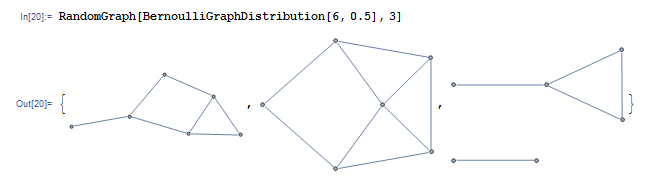
\includegraphics[width=\textwidth]{figures/mathematica-random.png}}
\caption{Mathematica function to generate three graphs}
\end{figure}

    %\todo{Directed graphs, different types of graphs}

    A list of relevent graph distributions is as follows.

    \begin{itemize}
    \item
    \code{BernoulliGraphDistribution[n, p]} generates $n$ vertices and a $p$ chance of an edge occuring between them. This is the random edge generation method decribed above where a fixed amount of vertices will be generated and every pair of vertices will have a probability of an edge occuring between them.

    \item 
    \code{UniformGraphDistribution[n, m]} generates a uniform graph distribution on $n$ vertices and $m$ edges. This distribution is equivilent to the random edge selection method above where there are a fixed number of vertices and edges but the positions of the edges are random generated.

    \item 
    \code{BarabasiAlbertGraphDistribution[n, k]} generates $n$ vertices where a new vertex with $k$ edges is added at each step. This distribution will force each vertex to have at least $k$ edges attached to it.

    \item
    \code{PriceGraphDistribution[n, k, a]} generates a graph with a de Solla Price distribution which is a distribution that gives edges a preferential attachment to vertices.

    \item
    \code{DegreeGraphDistribution[dlist]} generates a graph where $\mathrm{vertex}_i$ has degree $\mathrm{dlist}_i$.
    \end{itemize}

    Additionally the user can use the progamming language to programatically generate a graph based on his own method. There exists functions \code{EdgeAdd} and \code{VertexAdd} which can be combined with some random functions. In the next example, \code{StarGraph[n]} is used which constructs a graph with $n$ vertices with one vertex connected to all others. Next an edge is added onto this graph between $v_2$ and $v_r$ where $v_i$ is vertex $i$ and $r$ is a random number in the range $\{0,...,10\}$.

    \begin{figure}[htb]
\centering
\setlength\fboxsep{0pt}
\setlength\fboxrule{0.5pt}
\fcolorbox{lightgray}{white}{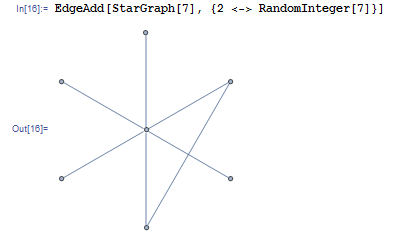
\includegraphics[scale=0.8]{figures/mathematica-star.png}}
\caption{Mathematica function to generate a star}
\end{figure}

    This shows that Mathematica gives the user a powerful set of tools and multiple methods of generating random graphs. However there is no general solution for generating random graphs, the user must learn the programming language and must have a specific algorithm in mind. For anything more advanced than adding specific edges or nodes, the code can get very complex.

    The output graph will be immediately shown to the user and more processing can be done on it. Additionally the data of this graph can be exported in a number of largely used formats including \emph{GraphML}, \emph{GXL}, \emph{Graph6}, \emph{DOT}. Furthermore, the generated image of the graph can be saved for the user to use in documents.

\subsection{Hypergraph Languages}
  \subsubsection{Hyperedge Replacement}

    It is possible to construct new hypergraphs by the replacement of a hyperedge by a new hypergraph to yield a new hypergraph. A hyperedge $e$ in a hypergraph $H$ may be replaced with another hypergraph $R$. An sequence of external nodes $ext$ in $R$ is needed where each node in $ext$ corresponds to an attachment node of $e$.

    A \emph{hypergraph with external nodes} is defined as a pair $\langle H, ext \rangle$ where $H$ is a hypergraph and $ext \in V_H*$ is a \emph{sequence} of external nodes. The set of external nodes is denoted by $EXT$.

    A replacement happens by first removing the hyperedge $e$, then adding the hypergraph $R$ excluding external nodes. Then for each hyperedge in $R$ that points to an external node, the tentacle must now point to the corresponding attachment nodes of $e$.

    The definition of hyperedge replacement is as follows:

    Let $\langle H, ext_H \rangle$, $\langle R, ext_R \rangle$ be disjoint hypergraphs with external nodes. $e$ is a hyperedge in $H$ where $type(e) = |ext_R|$. The replacement of hyperedge $e$ in a hypergraph with external nodes $H$ with the a hypergraph with external nodes $R$ is denoted by $\langle H, ext_H \rangle[e/\langle R, ext_R\rangle] = \langle X, ext_X \rangle$, also written $H[e/R] = X$ where the sequence of external nodes are implied. 

    \todo{Context-free Hypergraph Grammars: Node and Hyperedge Rewriting}

    \begin{align*}
    V_X &= V_H \cup (V_R \setminus EXT_R) \\[2mm]
    E_X &= (E_H \setminus \{e\}) \cup E_R \\[2mm]
    lbl_X(e') &= \begin{dcases*}
      lbl_H(e') \textrm{ if } e' \in E_H \setminus {e} \\
      lbl_R(e') \textrm{ if } e' \in E_R
    \end{dcases*} \\[2mm]
    att_X(e', i) &= \begin{dcases*}
      att_H(e', i) \textrm{ if } e' \in E_H \setminus {e} \\
      att_H(e, j) \textrm{ if } e' \in E_R \textrm{ and } att_R(e', i) = ext_R(j) \\
      att_R(e', i) \textrm{ if } e' \in E_R \textrm{ and } att_R(e', i) \in (V_R \setminus EXT_R)
    \end{dcases*} \\
    &\ \textrm{for } i \in 1..type(e') \\[2mm]
    ext_X &= ext_H
    \end{align*}

    We can see an example of hyperedge replacement here.
    
    \begin{figure}[H]
  \centering
  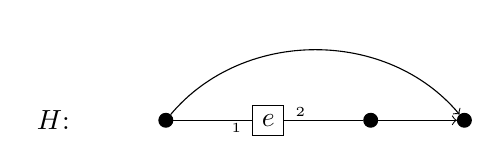
\begin{tikzpicture}

    \node (lbl) {$H$:};
    \node[vertex,right=of lbl] (a) {};
    \node[hyperedge] (hyp) [right=of a] {$e$};
    \node[vertex] (b) [right=of hyp] {};
    \node[vertex] (c) [right=of b] {};


    \path[->] (a) edge [bend left=50] (c)
              (b) edge (c);

    \path[-] (hyp) edge node[tentacle]{$1$} (a)
                   edge node[tentacle]{$2$} (b);

  \end{tikzpicture} \\[0.5cm]
  
  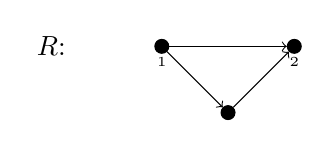
\begin{tikzpicture}

    \node (lbl) {$R$:};
    \node[vertex] (a) [right=of lbl] {} node[below=0mm of a,font=\tiny,inner sep=1pt]{1};
    \node[vertex] (b) [below right=1cm of a] {};
    \node[vertex] (c) [above right=1cm of b] {} node[below=0mm of c,font=\tiny,inner sep=1pt]{2};

    \path[->] (a) edge (b)
                  edge (c)
              (b) edge (c);
  \end{tikzpicture} \\[0.5cm]
  
  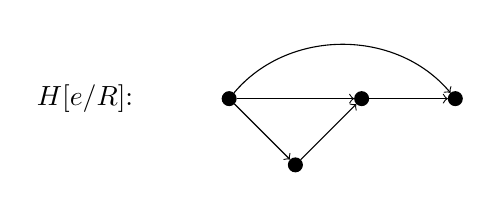
\begin{tikzpicture}

    \node (lbl) {$H[e/R]$:};
    \node[vertex,right=of lbl] (a) {};
    \node[vertex] (b) [below right=1cm of a] {};
    \node[vertex] (c) [above right=1cm of b] {};
    \node[vertex] (d) [right=of c] {};

    \path[->] (a) edge [bend left=50] (d)
                  edge (b)
                  edge (c)
              (b) edge (c)
              (c) edge (d);

  \end{tikzpicture}
  \caption{Hyperedge replacement}
\end{figure}

    A couple of properties can be observed in hyperedge replacement. Firstly, the sequentialization and parallelization property. Given two different replacements, the result will be equivilent whether the replacements happen one after another or simultaneously.

    \begin{equation}
    H[e_1/H_1,...e_n/H_n] = H[e_1/H_1]...[e_n/H_n]
    \end{equation}

    Secondly the replacement is confluent, this means hyperedges in a hypergraph can be replaced in any order without affecting the result.

    \begin{equation}
    H[e_1/H_1][e_2/H_2] = H[e_2/H_2][e_1/H_1]
    \end{equation}

    Finally we know the replacement is associative. If a hyperedge is replaced and then a part of the new hypergraph is replaced, this is equivilent to replacing the second hyperedge and then replacing the first hyperedge with the result.

    \begin{equation}
    H[e_1/H_1][e_2/H_2] = H[e_1/H_1 [e_2/H_2]]
    \end{equation}

  \subsubsection{Hyperedge Replacement Grammars}

    Hypergraphs can be generated using productions based on hyperedge replacement. A production is $p = x \to \langle R, ext \rangle$ where $x$ is a non-terminal so let $H$, $H'$ be hypergraphs and let $e \in E_H$ such that $l_{H}(e) = x$. Then $H$ directly derives $H'$ by $p$ applied to $e$ if $H'$ is equivilent to $H[e / R]$. This can be written $H \underset{p}{\Rightarrow} H'$.

    If we are given a production:
    \begin{figure}[H]
  \centering
  
  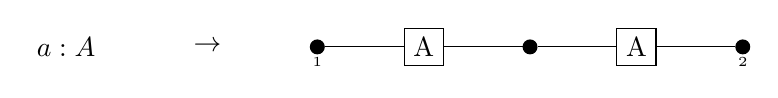
\begin{tikzpicture}

    \node[] (lbl) [] {$a: A$};


    \node[] (arrow1) [right=of lbl] {$\to$};


    \node[vertex] (a) [right=of arrow1] {} node[below=0mm of a,font=\tiny,inner sep=1pt]{1};
    \node[hyperedge] (hyp1) [right=of a] {A};
    \node[vertex] (b) [right=of hyp1] {};
    \node[hyperedge] (hyp2) [right=of b] {A};
    \node[vertex] (c) [right=of hyp2] {} node[below=0mm of c,font=\tiny,inner sep=1pt]{2};

    \path[-] (hyp1) edge node[tentacle]{} (a)
                   edge node[tentacle]{} (b);

    \path[-] (hyp2) edge node[tentacle]{} (b)
                   edge node[tentacle]{} (c);

    %\node[vertex] (a) [right=of arrow1] {} node[below=0mm of a,font=\tiny,inner sep=1pt]{1};
    %\node[vertex] (b) [below right=1cm of a] {};
    %\node[vertex] (c) [above right=1cm of b] {} node[below=0mm of c,font=\tiny,inner sep=1pt]{2};

    %\path[->] (a) edge (b)
    %              edge (c)
    %          (b) edge (c);
  \end{tikzpicture}
  
\end{figure}

    Then it follows:
    \begin{figure}[H]
  \centering
  
  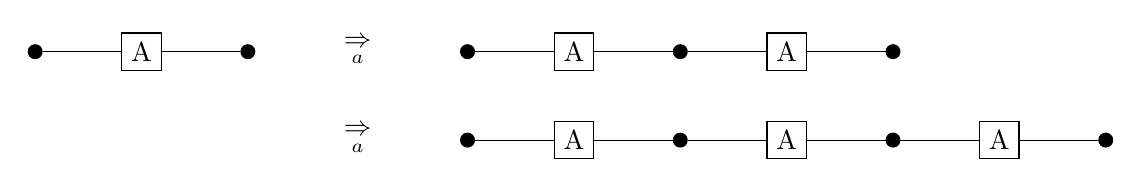
\begin{tikzpicture}

    \node[vertex] (a) [] {};
    \node[hyperedge] (hyp1) [right=of a] {A};
    \node[vertex] (b) [right=of hyp1] {};

    \path[-] (hyp1) edge node[tentacle]{} (a)
                   edge node[tentacle]{} (b);

    \node[] (arrow1) [right=of b] {$\underset{a}{\Rightarrow}$};

    \node[vertex] (a) [right=of arrow1] {};
    \node[hyperedge] (hyp1) [right=of a] {A};
    \node[vertex] (b) [right=of hyp1] {};
    \node[hyperedge] (hyp2) [right=of b] {A};
    \node[vertex] (c) [right=of hyp2] {};

    \path[-] (hyp1) edge node[tentacle]{} (a)
                   edge node[tentacle]{} (b);

    \path[-] (hyp2) edge node[tentacle]{} (b)
                   edge node[tentacle]{} (c);

   \node[] (arrow2) [below=0.5cm of arrow1] {$\underset{a}{\Rightarrow}$};

    \node[vertex] (a) [right=of arrow2] {};
    \node[hyperedge] (hyp1) [right=of a] {A};
    \node[vertex] (b) [right=of hyp1] {};
    \node[hyperedge] (hyp2) [right=of b] {A};
    \node[vertex] (c) [right=of hyp2] {};
    \node[hyperedge] (hyp3) [right=of c] {A};
    \node[vertex] (d) [right=of hyp3] {};

    \path[-] (hyp1) edge node[tentacle]{} (a)
                   edge node[tentacle]{} (b);

    \path[-] (hyp2) edge node[tentacle]{} (b)
                   edge node[tentacle]{} (c);

    \path[-] (hyp3) edge node[tentacle]{} (c)
                   edge node[tentacle]{} (d);

  \end{tikzpicture}
  
\end{figure}

    A hyperedge replacement grammar (HR grammar) is a system for generating a hypergraph language through a set of derivations. It is similar to other language generation concepts in computer science.

    A HR grammar can be defined as $G = \langle N, T, P, S \rangle$ where $N$ is a set of non-terminals, $T$ is a set of terminals disjoint with $N$, $S$ is the start graph. $P$ is a set of productions which are in the form of $x \to \langle R, ext \rangle$ where $x \in N$, $R$ is a hypergraph and $ext$ is the sequence of external nodes in $R$.

    The language of a control flow graph can be generated with the following
    \tikzset{
    every node/.style={scale=0.8,node distance=0.8cm and 0.6cm,anchor=center},
    seperator/.style={color=lightgray},
    aligned/.style={
      to path={
        (\tikztostart) -| (\tikztotarget)
        \tikztonodes
      }
    },
    bent left down/.style={
      to path={
        -- +(-0.5cm,0) .. controls +(-0.5,-0.5) and +(-0.5,0.2) ..  (\tikztotarget) \tikztonodes
      }},
    bent right down/.style={
      to path={
        -- +(0.5cm,0) .. controls +(0.5,-0.5) and +(0.5,0.2) ..  (\tikztotarget) \tikztonodes
      }},
    bent left up/.style={
      to path={
        -- +(-0.5cm,0) .. controls +(-0.5,0.5) and +(-0.5,-0.2) ..  (\tikztotarget) \tikztonodes
      }},
    bent right up/.style={
      to path={
        -- +(0.5cm,0) .. controls +(0.5,0.5) and +(0.5,-0.2) ..  (\tikztotarget) \tikztonodes
      }},
    bent right up big/.style={
      to path={
        -- +(0.5cm,0) .. controls +(0.5,1) and +(1,-0.2) ..  (\tikztotarget) \tikztonodes
      }},
    bent left up big/.style={
      to path={
        -- +(-0.5cm,0) .. controls +(-0.5,1) and +(-1,-0.2) ..  (\tikztotarget) \tikztonodes
      }},
    dhyperedge/.style={hyperedge,diamond},
    dbelow/.style={below=#1.center,anchor=center},
    dbelow2/.style={below=1.6 #1.center,anchor=center},
    dbelow3/.style={below=2.4 #1.center,anchor=center},
    dbelow4/.style={below=3.2 #1.center,anchor=center},
    dbelow left/.style={below left=#1.center,anchor=center},
    dbelow left2/.style={below left=1.6 and 0.6 #1.center,anchor=center},
    dbelow left3/.style={below left=2.4 and 0.6 #1.center,anchor=center},
    dbelow right/.style={below right=#1.center,anchor=center},
    dbelow right2/.style={below right=1.6 and 0.6 #1.center,anchor=center},
    dbelow right3/.style={below right=2.4 and 0.6 #1.center,anchor=center},
  }

\begin{figure}[H]
  \centering
  

  

  \begin{tikzpicture}[scale=0.5,node distance=0.5cm]

    \matrix[column sep=0.5cm]
    {
    \node (lbl) {$C \to $};

    &

    \node[vertex]     (a)    [label=1] {};
    \node[hyperedge]  (hyp1) [dbelow=of a] {$C$};
    \node[vertex]     (b)    [dbelow=of hyp1] {};
    \node[hyperedge]  (hyp2) [dbelow=of b] {$C$};
    \node[vertex]     (c)    [dbelow=of hyp2,label=2] {} ;

    \path[-] (hyp1) edge node[tentacle]{$1$} (a)
                    edge node[tentacle]{$2$} (b)
             (hyp2) edge node[tentacle]{$1$} (b)
                    edge node[tentacle]{$2$} (c);

    &
      \draw[seperator] (0,0) -- (0,-3.2);
    &

    \node[vertex]     (a)    [label=1] {};
    \node[dhyperedge] (hyp1) [dbelow2=of a] {$D$};
    \node[vertex]     (b)    [dbelow2=of hyp1,label=2] {};

    \path[-] (hyp1) edge node[tentacle]{$1$} (a)
                    edge[bent left down] node[tentacle]{$2$} (b) 
                    edge[bent right down] node[tentacle]{$3$} (b);


    &
      \draw[seperator] (0,0) -- (0,-3.2);
    &
    
    \node[vertex]     (a)    [label=1] {};
    \node[dhyperedge] (hyp1) [dbelow2=of a] {$D$};
    \node[vertex]     (b)    [dbelow2=of hyp1,label=2] {};

    \path[-] (hyp1) edge node[tentacle]{$1$} (a)
                    edge[bent left up] node[tentacle]{$2$} (a) 
                    edge[bent right down] node[tentacle]{$3$} (b);

    &
      \draw[seperator] (0,0) -- (0,-3.2);
    &
    
    \node[vertex]     (a)    [label=1] {};
    \node[dhyperedge] (hyp1) [dbelow2=of a] {$D$};
    \node[vertex]     (b)    [dbelow2=of hyp1,label=2] {};

    \path[-] (hyp1) edge node[tentacle] {$1$} (a)
                    edge[bent left down] node[tentacle] {$2$} (b) 
                    edge[bent right up] node[tentacle] {$3$} (a);
    
    &
      \draw[seperator] (0,0) -- (0,-3.2);
    &

    \node[vertex]     (a)    [label=1] {};
    \node[hyperedge]  (hyp1) [dbelow2=of a] {$c$};
    \node[vertex]     (b)    [dbelow2=of hyp1,label=2] {};

    \path[-] (hyp1) edge node[tentacle]{$1$} (a)
                    edge node[tentacle]{$2$} (b);
    \\
    };
  \end{tikzpicture} \\[1cm]

  \begin{tikzpicture}[scale=0.1,node distance=0.5cm]
    \matrix[column sep=0.5cm,row sep=1cm]
    {

    \node (lbl) {$D \to $};

    &

    \node[vertex]     (a)    [label=1] {};
    \node[dhyperedge] (hyp1) [dbelow=of a] {$D$};
    \node[vertex]     (b)    [dbelow right=of hyp1] {};
    \node[hyperedge]  (hyp2) [dbelow=of b] {$C$};
    \node[vertex]     (d)    [dbelow=of hyp2,label=3] {};
    \node[vertex]     (c)    [dbelow left3=of hyp1,label=2] {};

    \path[-] (hyp1) edge node[tentacle]{$1$} (a)
                    edge[aligned] node[tentacle]{$2$} (c) 
                    edge[aligned] node[tentacle]{$3$} (b)
             (hyp2) edge node[tentacle]{$1$} (b)
                    edge node[tentacle]{$2$} (d);


    &
      \draw[seperator] (0,0) -- (0,-3.2);
    &

    \node[vertex]     (a)    [label=1] {};
    \node[dhyperedge] (hyp1) [dbelow=of a] {$D$};
    \node[vertex]     (b)    [dbelow left=of hyp1] {};
    \node[hyperedge]  (hyp2) [dbelow=of b] {$C$};
    \node[vertex]     (c)    [dbelow=of hyp2,label=2] {};
    \node[vertex]     (d)    [dbelow right3=of hyp1,label=3] {};

    \path[-] (hyp1) edge node[tentacle]{$1$} (a)
                    edge[aligned] node[tentacle]{$2$} (b)
                    edge[aligned] node[tentacle]{$3$} (d)
             (hyp2) edge node[tentacle]{$1$} (b)
                    edge node[tentacle]{$2$} (c);

    &
      \draw[seperator] (0,0) -- (0,-3.2);
    &

    \node[vertex]     (a)    [label=1] {};
    \node[dhyperedge] (hyp1) [dbelow=of a] {$D$};
    \node[vertex]     (b)    [dbelow left=of hyp1] {};
    \node[dhyperedge] (hyp2) [dbelow=of b] {$D$};
    \node[vertex]     (c)    [dbelow right=of hyp2,label=2] {};
    \node[vertex]     (d)    [dbelow right3=of hyp1,label=3] {};

    \path[-] (hyp1) edge node[tentacle]{$1$} (a)
                    edge[aligned] node[tentacle]{$2$} (b) 
                    edge[aligned] node[tentacle]{$3$} (d)
             (hyp2) edge node[tentacle]{$1$} (b)
                    edge[bent left up big] node[tentacle]{$2$} (a)
                    edge[aligned] node[tentacle]{$3$} (c);
    
    &
      \draw[seperator] (0,0) -- (0,-3.2);
    &

    \node[vertex]     (a)    [label=1] {};
    \node[dhyperedge] (hyp1) [dbelow=of a] {$D$};
    \node[vertex]     (b)    [dbelow right=of hyp1] {};
    \node[dhyperedge] (hyp2) [dbelow=of b] {$D$};
    \node[vertex]     (c)    [dbelow left3=of hyp1,label=2] {};
    \node[vertex]     (d)    [dbelow left=of hyp2,label=3] {};

    \path[-] (hyp1) edge node[tentacle]{$1$} (a)
                    edge[aligned] node[tentacle]{$2$} (c) 
                    edge[aligned] node[tentacle]{$3$} (b)
             (hyp2) edge node[tentacle]{$1$} (b)
                    edge[aligned] node[tentacle]{$2$} (d)
                    edge[bent right up big] node[tentacle]{$3$} (a);

    &
      \draw[seperator] (0,0) -- (0,-3.2);
    

    \\

    &
    
    \node[vertex]     (a)    [label=1] {};
    \node[dhyperedge] (hyp1) [dbelow=of a] {$D$};
    \node[vertex]     (b)    [dbelow right=of hyp1] {};
    \node[dhyperedge] (hyp2) [dbelow=of b] {$D$};
    \node[vertex]     (c)    [dbelow left=of hyp2,label=2] {};
    \node[vertex]     (d)    [dbelow right=of hyp2,label=3] {};

    \path[-] (hyp1) edge node[tentacle]{$1$} (a)
                    edge[bent left down] node[tentacle]{$2$} (c) 
                    edge[aligned] node[tentacle]{$3$} (b)
             (hyp2) edge node[tentacle]{$1$} (b)
                    edge[aligned] node[tentacle]{$2$} (c)
                    edge[aligned] node[tentacle]{$3$} (d);

    
    &
      \draw[seperator] (0,0) -- (0,-3.2);
    &

    \node[vertex]     (a)    [label=1] {};
    \node[dhyperedge] (hyp1) [dbelow=of a] {$D$};
    \node[vertex]     (b)    [dbelow left=of hyp1] {};
    \node[dhyperedge] (hyp2) [dbelow=of b] {$D$};
    \node[vertex]     (c)    [dbelow left=of hyp2,label=2] {};
    \node[vertex]     (d)    [dbelow right=of hyp2,label=3] {};

    \path[-] (hyp1) edge node[tentacle]{$1$} (a)
                    edge[aligned] node[tentacle]{$2$} (b) 
                    edge[bent right down] node[tentacle]{$3$} (d)
             (hyp2) edge node[tentacle]{$1$} (b)
                    edge[aligned] node[tentacle]{$2$} (c)
                    edge[aligned] node[tentacle]{$3$} (d);


    &
      \draw[seperator] (0,0) -- (0,-3.2);
    &

    \node[vertex]     (a)     [anchor=center,label=1] {};
    \node[hyperedge]  (hyp1)  [dbelow=of a] {$C$};
    \node[vertex]     (b)     [dbelow=of hyp1] {};
    \node[dhyperedge] (hyp2)  [dbelow=of b] {$D$};
    \node[vertex]     (c)     [dbelow left=of hyp2,label=2] {};
    \node[vertex]     (d)     [dbelow right=of hyp2,label=3] {};

    \path[-] (hyp1) edge node[tentacle]{$1$} (a)
                    edge node[tentacle]{$2$} (b)
             (hyp2) edge node[tentacle]{$1$} (b)
                    edge[aligned] node[tentacle]{$2$} (c) 
                    edge[aligned] node[tentacle]{$3$} (d);
    
    &
      \draw[seperator] (0,0) -- (0,-3.2);
    &

    \node[vertex]     (a)    [label=1] {};
    \node[dhyperedge] (hyp1) [dbelow=of a] {$d$};
    \node[vertex]     (b)    [dbelow left3=of hyp1,label=2] {};
    \node[vertex]     (c)    [dbelow right3=of hyp1,label=3] {};

    \path[-] (hyp1) edge node[tentacle]{$1$} (a)
                    edge[aligned] node[tentacle]{$2$} (b) 
                    edge[aligned] node[tentacle]{$3$} (c);

    \\
    };
  \end{tikzpicture}

  


  \caption{Flowchart grammar}
  
\end{figure}
\begin{figure}[H]
  \centering

  \begin{tikzpicture}

    \matrix[column sep=1cm,row sep=1cm]
    {
      \node[vertex]     (a)    [label=1] {};
      \node[hyperedge]  (hyp1) [dbelow2=of a] {$C$};
      \node[vertex]     (b)    [dbelow2=of hyp1,label=2] {};

      \path[-] (hyp1) edge node[tentacle]{$1$} (a)
                      edge node[tentacle]{$2$} (b);

      &
      \node[]           (arrow) [] {$\Rightarrow$};
      &

      \node[vertex]     (a)    [label=1] {};
      \node[dhyperedge] (hyp1) [dbelow2=of a] {$D$};
      \node[vertex]     (b)    [dbelow2=of hyp1,label=2] {};

      \path[-] (hyp1) edge node[tentacle]{$1$} (a)
                      edge[bent left down] node[tentacle]{$2$} (b) 
                      edge[bent right down] node[tentacle]{$3$} (b);

      &
      \node[]           (arrow) [] {$\Rightarrow$};
      &

      \node[vertex]     (a)    [label=1] {};
      \node[dhyperedge] (hyp1) [dbelow=of a] {$D$};
      \node[vertex]     (b)    [dbelow right=of hyp1] {};
      \node[dhyperedge] (hyp2) [dbelow=of b] {$D$};
      \node[vertex]     (c)    [dbelow left=of hyp2,label=2] {};

      \path[-] (hyp1) edge node[tentacle]{$1$} (a)
                      edge[bent left down] node[tentacle]{$2$} (c) 
                      edge[aligned] node[tentacle]{$3$} (b)
               (hyp2) edge node[tentacle]{$1$} (b)
                      edge[aligned] node[tentacle]{$2$} (c)
                      edge[bent right up big] node[tentacle]{$3$} (a);
      &
      \node[]           (arrow) [] {$\Rightarrow$};
      &


      \node[vertex]     (a)    [label=1] {};
      \node[hyperedge]  (hyp1) [dbelow=of a] {$C$};
      \node[vertex]     (b)    [dbelow=of hyp1] {};
      \node[dhyperedge] (hyp2) [dbelow=of b] {$D$};
      \node[vertex]     (c)    [dbelow right=of hyp2] {};
      \node[dhyperedge] (hyp3) [dbelow=of c] {$D$};
      \node[vertex]     (d)    [dbelow left=of hyp3,label=2] {};

      \path[-] (hyp1) edge node[tentacle]{$1$} (a)
                      edge node[tentacle]{$2$} (b)
               (hyp2) edge node[tentacle]{$1$} (b)
                      edge[bent left down] node[tentacle]{$2$} (d) 
                      edge[aligned] node[tentacle]{$3$} (c)
               (hyp3) edge node[tentacle]{$1$} (c)
                      edge[aligned] node[tentacle]{$2$} (d)
                      edge[bent right up big] node[tentacle]{$3$} (a);
      
      \\
      &
      \node[]           (arrow) [] {$\Rightarrow$};
      &


      \node[vertex]     (a)    [label=1] {};
      \node[hyperedge]  (hyp1) [dbelow=of a] {$C$};
      \node[vertex]     (b)    [dbelow=of hyp1] {};
      \node[dhyperedge] (hyp2) [dbelow=of b] {$D$};
      \node[vertex]     (c)    [dbelow right=of hyp2] {};
      \node[dhyperedge] (hyp3) [dbelow=of c] {$D$};
      \node[vertex]     (d)    [dbelow left=of hyp3,label=2] {};
      \node[hyperedge]  (hyp4) [dbelow=of d] {$C$};
      \node[vertex]     (e)    [dbelow=of hyp4] {};

      \path[-] (hyp1) edge node[tentacle]{$1$} (a)
                      edge node[tentacle]{$2$} (b)
               (hyp2) edge node[tentacle]{$1$} (b)
                      edge[bent left down] node[tentacle]{$2$} (e) 
                      edge[aligned] node[tentacle]{$3$} (c)
               (hyp3) edge node[tentacle]{$1$} (c)
                      edge[aligned] node[tentacle]{$2$} (d)
                      edge[bent right up big] node[tentacle]{$3$} (a)
               (hyp4) edge node[tentacle]{$1$} (d)
                      edge node[tentacle]{$2$} (e);

      &
      \node[]           (arrow) [] {$\Rightarrow$};
      &


      \node[vertex]     (a)    [label=1] {};
      \node[hyperedge]  (hyp1) [dbelow=of a] {$C$};
      \node[vertex]     (b)    [dbelow=of hyp1] {};
      \node[dhyperedge] (hyp2) [dbelow=of b] {$D$};
      \node[vertex]     (c)    [dbelow right=of hyp2] {};
      \node[dhyperedge] (hyp3) [dbelow=of c] {$D$};
      \node[vertex]     (d)    [dbelow left=of hyp3,label=2] {};
      \node[hyperedge]  (hyp4) [dbelow=of d] {$C$};
      \node[vertex]     (e)    [dbelow=of hyp4] {};
      \node[vertex]     (f)    [dbelow left=of hyp2] {};
      \node[hyperedge]  (hyp5) [dbelow=of f] {$C$};

      \path[-] (hyp1) edge node[tentacle]{$1$} (a)
                      edge node[tentacle]{$2$} (b)
               (hyp2) edge node[tentacle]{$1$} (b)
                      edge[aligned] node[tentacle]{$2$} (f) 
                      edge[aligned] node[tentacle]{$3$} (c)
               (hyp3) edge node[tentacle]{$1$} (c)
                      edge[aligned] node[tentacle]{$2$} (d)
                      edge[bent right up big] node[tentacle]{$3$} (a)
               (hyp4) edge node[tentacle]{$1$} (d)
                      edge node[tentacle]{$2$} (e)
               (hyp5) edge node[tentacle]{$1$} (f);
      \draw (hyp5) .. controls +(0,-0.5) and +(-0.5,0.2) .. (e) node[tentacle]{$2$};

      &
      \node[]           (arrow) [] {$\Rightarrow^{*}$};
      &


      \node[vertex]     (a)    [label=1] {};
      \node[hyperedge]  (hyp1) [dbelow=of a] {$c$};
      \node[vertex]     (b)    [dbelow=of hyp1] {};
      \node[dhyperedge] (hyp2) [dbelow=of b] {$d$};
      \node[vertex]     (c)    [dbelow right=of hyp2] {};
      \node[dhyperedge] (hyp3) [dbelow=of c] {$d$};
      \node[vertex]     (d)    [dbelow left=of hyp3,label=2] {};
      \node[hyperedge]  (hyp4) [dbelow=of d] {$c$};
      \node[vertex]     (e)    [dbelow=of hyp4] {};
      \node[vertex]     (f)    [dbelow left=of hyp2] {};
      \node[hyperedge]  (hyp5) [dbelow=of f] {$c$};

      \path[-] (hyp1) edge node[tentacle]{$1$} (a)
                      edge node[tentacle]{$2$} (b)
               (hyp2) edge node[tentacle]{$1$} (b)
                      edge[aligned] node[tentacle]{$2$} (f) 
                      edge[aligned] node[tentacle]{$3$} (c)
               (hyp3) edge node[tentacle]{$1$} (c)
                      edge[aligned] node[tentacle]{$2$} (d)
                      edge[bent right up big] node[tentacle]{$3$} (a)
               (hyp4) edge node[tentacle]{$1$} (d)
                      edge node[tentacle]{$2$} (e)
               (hyp5) edge node[tentacle]{$1$} (f);
      \draw (hyp5) .. controls +(0,-0.5) and +(-0.5,0.2) .. (e) node[tentacle]{$2$};


      \\
    };
  \end{tikzpicture}
  \caption{Example derivation of flowchart grammar}
\end{figure}

\subsection{Ranjan's Approach}
  In order to generate random graphs we can study Ranjan's approach to graph generation. Ranjan\cite{Ranjan} decribes a method of generating a random sequence of productions over a graph grammar $G$ which can then be run to generate a single random graph.

  There are two seperate stages in Ranjan's approach that will henceforth be known as the `generation stage' and the `run stage'. Firstly, the generation stage will generate a sequence of rules and locations and the run stage will actually perform this sequence of replacement rules i.e productions.

  \begin{itemize}
  \item Firstly, $n_1$ is initialised to contain all the available locations based on the start graph.
  \item For each rule in the grammar, the number of available locations that the rule adds must be calculated (See below for definition of available location.)
  \item Begin looping $i = 1,2...$
  \item The system will generate a random integer $1 \leq m \leq \#P$ which is for identifying which rule is chosen. Another random integer $1 \leq l \leq n_i$ is chosen to identify the location that the rule is applied to. The tuple $\langle m,l \rangle$ is added to the sequence of rules to be applied.
  \item Assign $n_{i+1} = n_i$ plus the number of additional locations added for rule $m$. 
  \item Repeat loop until some condition
  \end{itemize}

  The loop continues until some predetermined end condition. For example, we could restrict the number of edges/vertices, or restrict the number of iterations. If a range is given then the size is chosen randomly to make the graph even more random.

  \paragraph{}

  An `available' location is a node where \emph{all} productions can be applied. Because Ranjan's approach generates a complete list of rules and locations before actually performing any replacements, it does know the current state of the graph. When a rule $\langle m,l \rangle$ is performed, $l$ must always refer to a currently available location and it must always be possible for production $m$ to be performed on that location. For every graph in the language, there must be at least one available location and the number of available locations never decreases (consequently the language is infinite.) In Ranjan's examples every production adds zero or one new available location. Note that the grammar may produce nodes that one or more productions \emph{cannot} be matched, but these must not be considered `available'.
  
  Ranjan uses a language called GP (Graph Programs) to perform the sequence of rules but the actual system used is irrelevant and the replacements can be performed by any means. The only requirement is that the system must keep track of the available locations. In Ranjan's implementation, the grammar itself is modified to number the available nodes $1..N$ but it is equally valid to keep a sequence of these nodes seperate to the grammar.

  The result is a single graph and the process can be re-run to produce multiple random graphs. The drawbacks of this method is the strict set of rules placed on the grammar.

  \begin{figure}[!h]
  \centering
  \begin{tikzpicture}

    \matrix[column sep=2cm]
    {
    \node[vertex]     (lefta) [label=1] {};
    \node             (arrow) [right=of lefta] {$\underset{r_1}{\Rightarrow}$};
    \node[vertex]     (a)     [right=of arrow,label=1] {};
    \node[vertex]     (b)     [below=of a] {};

    \path[-] (a) edge (b);
    &

    \node[vertex]     (lefta) [label=1] {};
    \node             (arrow) [right=of lefta] {$\underset{r_2}{\Rightarrow}$};
    \node[vertex]     (a)     [right=of arrow,label=1] {};
    \node[vertex]     (b)     [node distance=1cm and 0.5cm,below left=of a] {};
    \node[vertex]     (c)     [node distance=1cm and 0.5cm,below right=of a] {};

    \path[-] (a) edge (b)
                 edge (c);
    \\
    };

  \end{tikzpicture}
  \caption{Binary tree grammar}

\end{figure}

  The figure below shows an example of the system applied to the binary tree grammar six times with a single node as the start graph and the number of iterations fixed at $5$.

  \begin{figure}[!h]
  \centering
  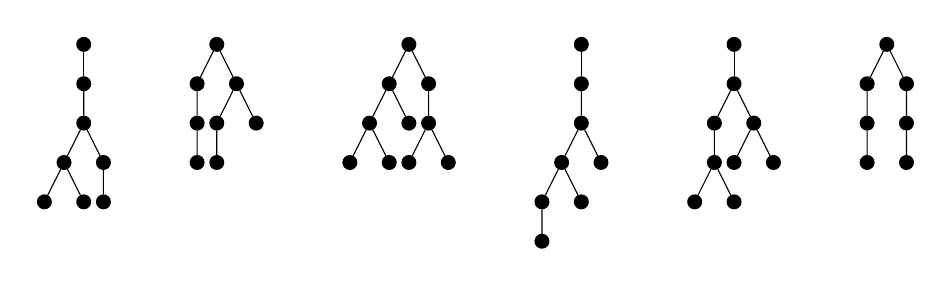
\begin{tikzpicture}[level distance=0.5cm,level/.style={sibling distance=0.5cm}]

    \matrix[column sep=1cm]
    {
      \node[vertex] {}
        child {node[vertex] {}
          child {node[vertex] {}
            child {node[vertex] {}
              child {node[vertex] {}}
              child {node[vertex] {}}
            }
            child {node[vertex] {}
              child {node[vertex] {}}
            }
          }
        };
    &
      \node[vertex] {}
        child {node[vertex] {}
          child {node[vertex] {}
            child {node[vertex] {}}
          }
        }
        child {node[vertex] {}
          child {node[vertex] {}
            child {node[vertex] {}}
          }
          child {node[vertex] {}}
        };
    &
      \node[vertex] {}
        child {node[vertex] {}
          child {node[vertex] {}
            child {node[vertex] {}}
            child {node[vertex] {}}
          }
          child {node[vertex] {}}
        }
        child {node[vertex] {}
          child {node[vertex] {}
            child {node[vertex] {}}
            child {node[vertex] {}}
          }
        };
    &
      \node[vertex] {}
        child {node[vertex] {}
          child {node[vertex] {}
            child {node[vertex] {}
              child {node[vertex] {}
                child {node[vertex] {}}
              }
              child {node[vertex] {}}
            }
            child {node[vertex] {}}
          }
        };
    &
      \node[vertex] {}
        child {node[vertex] {}
          child {node[vertex] {}
            child {node[vertex] {}
              child {node[vertex] {}}
              child {node[vertex] {}}
            }
          }
          child {node[vertex] {}
            child {node[vertex] {}}
            child {node[vertex] {}}
          }
        };
    &
      \node[vertex] {}
        child {node[vertex] {}
          child {node[vertex] {}
            child {node[vertex] {}}
          }
        }
        child {node[vertex] {}
          child {node[vertex] {}
            child {node[vertex] {}}
          }
        };
    \\
    };

  \end{tikzpicture}

\end{figure}

  In this figure we can see that both rules will match on leaf nodes due to the dangling condition. As such the system will need to mark just the leaf nodes as available nodes. It must also unmark nodes that become parent nodes. In $r_1$, the rule converts a leaf node into a parent node but also adds an available node, so the total available nodes increases by zero. On the other hand $r_2$ adds two new nodes so the total available nodes increases by one.

  The figure below shows an example of the system applied to the same grammar with the number of vertices bound $\leq 10$.
  \begin{figure}[!h]
  \centering
  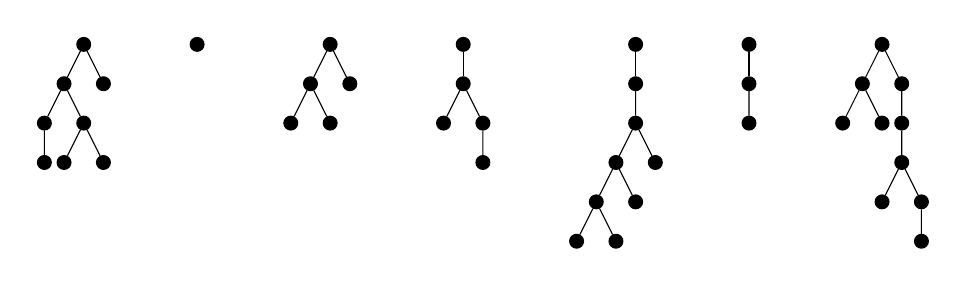
\begin{tikzpicture}[level distance=0.5cm,level/.style={sibling distance=0.5cm}]

    \matrix[column sep=1cm]
    {
      \node[vertex] {}
        child {node[vertex] {}
          child {node[vertex] {}
            child {node[vertex] {}}
          }
          child {node[vertex] {}
            child {node[vertex] {}}
            child {node[vertex] {}}
          }
        }
        child {node[vertex] {}};
    &
      \node[vertex] {};
    &
      \node[vertex] {}
        child {node[vertex] {}
          child {node[vertex] {}}
          child {node[vertex] {}}
        }
        child {node[vertex] {}};
    &
      \node[vertex] {}
        child {node[vertex] {}
          child {node[vertex] {}}
            child {node[vertex] {}
            child {node[vertex] {}}
          }
        };
    &
      \node[vertex] {}
        child {node[vertex] {}
          child {node[vertex] {}
            child {node[vertex] {}
              child {node[vertex] {}
                child {node[vertex] {}}
                child {node[vertex] {}}
              }
              child {node[vertex] {}}
            }
            child {node[vertex] {}}
          }
        };
    &
      \node[vertex] {}
        child {node[vertex] {}
          child {node[vertex] {}}
        };
    &
      \node[vertex] {}
        child {node[vertex] {}
          child {node[vertex] {}}
          child {node[vertex] {}}
        }
        child {node[vertex] {}
          child {node[vertex] {}
            child {node[vertex] {}
              child {node[vertex] {}}
              child {node[vertex] {}
                child {node[vertex] {}}
              }
            }
          }
        };
    \\
    };

  \end{tikzpicture}

\end{figure}


  \subsubsection{Improvement on Ranjan's Approach}

    It is likely that the reason Ranjan's approach happens in two stages is a workaround to GP which has a very simple instruction set. By changing the method keep a sequence of morphisms, we can improve it a bit.

    \begin{itemize}
    \item Let $d$ be a sequence of all isomorphic graph morphisms to $G$ for each rule in the grammar.
    \item Pick a random integer $1 \leq r \leq \#d$ and apply rule $d_r$ to the graph $G$.
    \item Update the sequence $d$
    \item Repeat loop until some condition
    \end{itemize}

    This method is a more general version of Ranjan's approach and there are no restrictions of the grammar. However, the implementation of this method is very expensive to compute since matching morphisms is not trivial.

    Another method is to use what we know about hypergraph languages. Below is a new method that works on hypergraphs. It keeps a sequence of available non-terminals and picks one at random. It then chooses a random rule that can be applied to this location and applies it the the graph. Using a sequence of non-terminals instead of graph morphisms gives a better computational speed since the lookup of non-terminals in a graph is a constant time operation.

    \begin{itemize}
    \item Let $G$ be the start graph. Let $d$ be a sequence of all the non-terminal hyperedges in $G$
    \item Begin loop
    \begin{itemize}
    \item Pick a random integer $1 \leq l \leq \#d$.
    \item Get the set of all valid rules on this edge. $r = \{\textrm{All rules $x \to \langle R, ext \rangle$ where $x = lbl_F(d_l)$\}}$
    \item Pick another random integer $1 \leq m \leq \#r$ and apply the rule $r_m$ to the graph $G$.
    \item Remove the non-terminal $d_l$ from $d$ and add all the non-terminals in the replaced graph $R$.
    \end{itemize}
    \item Repeat loop
    \end{itemize}

  \subsection{Hickey-Cohen Generation of Uniform Random Strings}

  The previous approach has a major downside that some terminal graphs have a far larger probability of occuring than others. Consider the string grammar $S \to a | Sa$, we can see here that the string $a$ has the probability $0.5$ of being produced and \emph{every} other terminal graph combined has the remaining probability of $0.5$. The same is true for graph grammars. A better option would be to choose terminal graphs with uniform randomness.

  The paper by Timothy Hickey and Jacques Cohen titled `Uniform Random Generation of Strings in a Context-Free Language' describes a method of picking strings uniformly. If the method can be constructed for strings we may be able to use the same method for graphs.

  The paper explains the meaning of producing strings uniformly - \emph{``Consider the set of all strings of length $n$ in the language. A uniform random generator is one which will produce strings from this set with equal probability.''} It is noted that the probability of which disjunct is used at each step in a derivation depends on the previous steps. This is different to the naive approach of choosing a derivation with equal probability and not taking into account the current state.

  Firstly some notation is introduced. Let $G = \langle V, \Sigma, P, N_1 \rangle$ be an unambiguous cycle-free context-free grammar containing no $\epsilon$-productions where $V = N \cup \Sigma$, $N = {N_1,\dots,N_r}$ is the nonterminal vocabulary, $\Sigma$ is the set of terminals, $N_1$ is the start symbol, and the set of productions is the following.
  \[P = \left\{\pi_{ij} : N_i \to \alpha_{ij} | i = 1,\dots,r, j = 1, \dots,s_i \right\}\]

  Choosing a string $\beta_{k+1}$ from a previous string $\beta_k$ involves rewriting the leftmost nonterminal in $\beta_k$ using one of the productions in $P$. If $N_i$ is the leftmost nonterminal in $B_k$, there are $s_i$ different choices for $\beta_{k+1}$. The idea of the method is to generate random strings of length $n$ by determining the probabilties $p_{ij}(\beta, n)$. These probabilities must be chosen so that every string of length $n$ has an equal probability.

  Let $g_\beta(n)$ denote the number of terminal strings of length $n$ that can be derived from a sentential form $\beta$ and $\gamma$ be the result of applying $\pi_{ij}$ to $\beta$ in a leftmost derivation. The probability that must be assigned to $\pi_{ij}$ is:
  \[
  p_{ij}(\beta, n) = \frac{g_\gamma(n)}{g_\beta(n)}
  \]
  A terminal string of length $n$ derived from the concatenation of two strings $\beta_1$, $\beta_2$ is the concatenation of two terminal strings whose lengths sum to $n$. The number of these terminal strings is the following.
  \[
  g_{\beta_1\beta_2}(n) = \sum_{n_1+n_2=n}g_{\beta_1}(n_1)g_{\beta_2}(n_2)
  \]
  This is in the form of a convolution $(g_{\beta_1} * g_{\beta_2})(n)$ which is defined as:
  \[
  (g_1 * g_2)(n) = \sum_{n_1+n_2=n}g_1(n_1)g_2(n_2) = \sum_{k=0}^{n} g_1(k)g_2(n-k)
  \]
  With the notation $g^{(k)}$ to denote the convolution of a function $g$ with itself $k$ times and were $\sum_{n_1+n_2=n}$ means all positive integer compositions $n_1$ and $n_2$ to add to $n$. The paper then shows the the associativity and commutativity properties of this convolution, as well as an `identity' function $\delta_k$ which is proved $\delta_0 * g = g$ and $g^{(0)} = \delta_0$
  \[
  \delta_k(n) = \left\{\begin{aligned}
    1, \quad & n = k\\
    0, \quad & n \neq k
  \end{aligned}\right.
  \]


  We can now define a function that calculates the number of terminal strings given a vector of nonterminals. This function is $f(t, a)$ for $a = (a_1,\dots,a_r)$ which corresponds to how many $N_1,\dots,N_r$ to count.
  \[
  f(t, a) = \left((g_{N_1}^{(a_1)}) * \hdots * (g_{N_r}^{(a_r)})\right)(t)
  \]
  Hickey and Cohen go on to show how this function can be rewritten as the following recurence
  \[
  f(t,a) = \sum_{j=1}^{s_i}f(t-T(\alpha_{ij}), a+A(\alpha_{ij})-A(N_i)), \quad\mathrm{if}\ a_i \neq 0
  \]

  Let $T(\beta)$ be the number of terminals in $\beta$ and let $A(\beta) = (A_1(\beta),\dots,A_r(\beta))$ be the vector whose $i$th component is the number of occurences of non-terminal $N_i$ in $\beta$. Then the function counting terminal strings from a string $\beta$ is the following.
  \[
  g_\beta(n) = f(n-T(\beta), A(\beta))
  \]

  Using this function we can rewrite the probability that production $\pi_{ij}$ will be used:
  \[
  p_{ij}(\beta, n) = \frac{f(n - T(\gamma), A(\gamma))}{f(n-T(\beta), A(\beta))} = \frac{f(n-T(\beta)-T(\alpha_{ij}),A(\beta)-A(N_i)+A(\alpha_{ij}))}{f(n-T(\beta),A(\beta))}
  \]

  The function $g_{N_i}$ can now be simplified.
  \begin{align*}
  g_{N_i}(t) &= f(t, A(N_i)) \\
  &= \sum_{j=1}^{s_i} f(t-T(\alpha_{ij}), A(\alpha_{ij})) \\
  &= \sum_{j=1}^{s_i} \left(g_{N_1}^{(\alpha_{ij})} * \hdots * g_{N_r}^{(\alpha_{rj})}\right)(t - T(\alpha_{ij})) \\
  \mathrm{with}\ g_{N_i}(t) &= 0\ \mathrm{if}\ t \leq 0
  \end{align*}

  This equation expresses $g(t)$ in terms of the values of $g_{N_i}(t')(1 \leq t' < t, 1 \leq i \leq r)$ so we can precompute the values $g_{N_i}(t)(1 \leq t \leq n, 1 \leq i \leq r)$ to speed up the generation of strings.

  \subsubsection{Example}

    Consider the following unambiguous context-free grammar that generates balances parentheses.
    \begin{align*}
    G_0 &= ({N_1, N_2, (, )}, {(, )}, P, N_1) \\
    P : \pi_{11} &: N_1 \to (N_1 \\
        \pi_{21} &: N_2 \to N_1 N_2 \\
        \pi_{22} &: N_2 \to\ )
    \end{align*}

    The method will compute the values of $g_{N_1}$ and $g_{N_2}$ for $1 \leq t \leq n$ using the formulas
    \begin{align*}
    g_{N_1}(t) &= g_{N_1}(t-1) \\
    g_{N_2}(t) &= (g_{N_1} * g_{N_2})(t) + (g_{N_1}^{(0)} * g_{N_2}^{(0)})(t-1) = (g_{N_1} * g_{N_2})(t) + \delta_0(t-1)
    \end{align*}

    \begin{figure}[H]
  \centering
  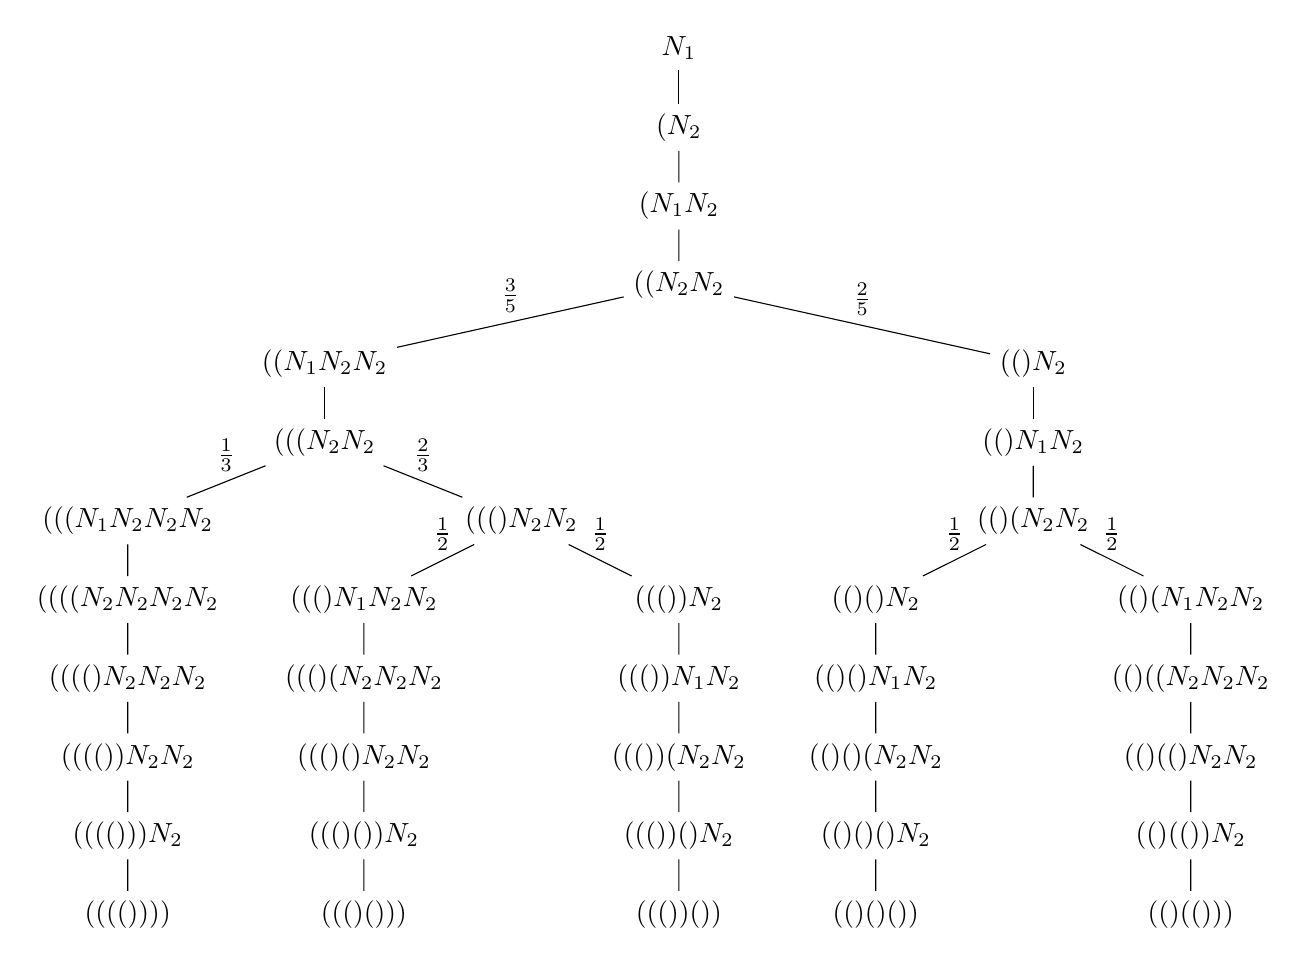
\begin{tikzpicture}[
    level distance=1cm,
    level 4/.style={sibling distance=9cm},
    level 6/.style={sibling distance=5cm},
    level 7/.style={sibling distance=4cm}]

  \node[] {$N_1$}
    child {node {$(N_2$}
      child {node {$(N_1N_2$}
        child {node {$((N_2N_2$}
          child {node {$((N_1N_2N_2$}
            child {node {$(((N_2N_2$}
              child {node {$(((N_1N_2N_2N_2$}
                child {node {$((((N_2N_2N_2N_2$}
                  child {node {$(((()N_2N_2N_2$}
                    child {node {$(((())N_2N_2$}
                      child {node {$(((()))N_2$}
                        child {node {$(((())))$}}
                      }
                    }
                  }
                }
                edge from parent         
                  node[above] {$\frac{1}{3}$}
              }
              child {node {$((()N_2N_2$}
                child {node {$((()N_1N_2N_2$}
                  child {node {$((()(N_2N_2N_2$}
                    child {node {$((()()N_2N_2$}
                      child {node {$((()())N_2$}
                        child {node {$((()()))$}}
                      }
                    }
                  }
                  edge from parent         
                    node[above] {$\frac{1}{2}$}
                }
                child {node {$((())N_2$}
                  child {node {$((())N_1N_2$}
                    child {node {$((())(N_2N_2$}
                      child {node {$((())()N_2$}
                        child {node {$((())())$}}
                      }
                    }
                  }
                  edge from parent         
                    node[above] {$\frac{1}{2}$}
                }
                edge from parent         
                  node[above] {$\frac{2}{3}$}
              }
            }
            edge from parent         
              node[above] {$\frac{3}{5}$}
          }
          child {node {$(()N_2$}
            child {node {$(()N_1N_2$}
              child {node {$(()(N_2N_2$}
                child {node {$(()()N_2$}
                  child {node {$(()()N_1N_2$}
                    child {node {$(()()(N_2N_2$}
                      child {node {$(()()()N_2$}
                        child {node {$(()()())$}}
                      }
                    }
                  }
                  edge from parent         
                    node[above] {$\frac{1}{2}$}
                }
                child {node {$(()(N_1N_2N_2$}
                  child {node {$(()((N_2N_2N_2$}
                    child {node {$(()(()N_2N_2$}
                      child {node {$(()(())N_2$}
                        child {node {$(()(()))$}}
                      }
                    }
                  }
                  edge from parent         
                    node[above] {$\frac{1}{2}$}
                }
              }
            }
            edge from parent         
              node[above] {$\frac{2}{5}$}
          }
        }
      }
    };
    
  \end{tikzpicture}
  \caption{Derivations tree with probabilties of strings of length 8}
\end{figure}


  \subsection{Combinatorics}

    
\section{Theory}

\subsection{Hickey-Cohen Generation of Hypergraphs}

  In this section, we will attempt to use the Hick Hickey-Cohen approach to generating uniform random strings to uniformly generate hypergraphs from a hypergraph grammar. 

  The function to calculate the number of terminal strings in a vector of  $f$ is expressed in terms of the functions $T(\beta)$ and $A(\beta)$ where $T(\beta)$ is the number of terminals in the string $\beta$ and $A(\beta)$ is a vector whose $i$th component is the number of occurences of $N_i$ in the string $\beta$. We must first redefine these functions for hypergraphs.

  Our grammar productions are named the same as before:
  \[P = \left\{\pi_{ij} : N_i \to \alpha_{ij} | i = 1,\dots,r, j = 1, \dots,s_i \right\}\]
  But instead of strings, now $N_1,\dots,N_r$ are non-terminal hyperedges and $\alpha_{ij}$ is the graph derivation.

  $A(\beta)$ is now a vector whose $i$th component is the number of occurences of the non-terminal edge $N_i$ in the grah $\beta$.

  In order to define $A(\beta)$ we must decide what `size' means for a hypergraph. This size must never decrease after applying a derivation and the following property must hold for derivations $d_1$ and $d_2$.
  \[
  T(\beta) + T(\alpha_{ij}) = T(\beta \Rightarrow \pi_{ij})
  \]
  What this means is when replacing a hyperedge with a subgraph ($\beta_1$), the overall size ($T(\beta)$) will increase by the size of the subgraph ($T(\beta_1)$).

  I have chosen the following where $t_\beta$ is the number of terminal hyperedges in graph $\beta$, $v_\beta$ is the number of vertices in the graph and $x_\beta$ is the number of external vertices in the graph.

  \[T(\beta) = t_\beta + v_\beta - x_\beta\]

  It is also possible to define $T(\beta)$ without non-terminal edges, so $T(\beta) = v_\beta - x_\beta$. The distiction is whether the user wants to limit number of vertices and terminal edges or just vertices. It is required to not count external nodes in this case, because these nodes get merged and the aforementioned property will not hold.

  The method now generates a graph of size $n$. To generate a single graph the program does the following.

  \begin{itemize}
    \item Start with a graph $\beta$ which is initial graph 
    \item For each non-terminal hyperedge in $\beta$ where the label of the hyperedge is $N_i$, the following sub-procedure must be done. This is repeated until there is no non-terminals left.

    It is worth noting that it doesn't matter which order the hyperedge is picked since it is known that hyperedge replacement can be performed in any order with the same output.
    \begin{itemize}
    \item Choose a production from the set $\left(\pi_{i1},\dots,\pi_{is_i}\right)$ by choosing a random number and using discrete cumulative probability distribution where production $\pi_{ij}$ has the probability $p_{ij}(\beta, n)$ of being chosen.

    For example, if the probabilities for $(\pi_{i1}, \pi_{i2}, \pi_{i2})$ are $(\frac{1}{2}, \frac{1}{4}, \frac{1}{4})$. A random number $0 \leq r \leq 1$ is used to choose the production $p$ accordingly. Therefore
    \[
    p = \left\{\begin{aligned}
      \pi_{i1}, \quad & r \le 0.5 \\
      \pi_{i2}, \quad & 0.5 < r \le 0.75 \\
      \pi_{i3}, \quad & 0.75 < r \le 1 \\
    \end{aligned}\right.
    \]
    The probability $\pi_{ij}$ may be zero in the case where applying this production can never produce a graph of size $n$. In this case the production should not be considered in the above choice.

    \item The production $p$ is applied the the graph $\beta$ which may add extra terminals and non-terminals.
    \end{itemize}

    \item $\beta$ is now a random graph of size $n$. 
  \end{itemize}

  If the user wants multiple graphs he can run this procedure as many times as needed.

\subsubsection{Example}

\begin{figure}[!h]
  \centering
  \begin{tikzpicture}
    \node             (lefta) {$N_1$};
    \node             (arrow) [right=of lefta] {$=$};
    \node[vertex]     (a)     [right=of arrow,label=1] {};
    \node[hyperedge]  (hyp1)  [below=0.5cm of a] {A};
    \path[-] (hyp1)   edge node[tentacle]{} (a);
  \end{tikzpicture}
  \caption{$N_1$ is the single non-terminal in our grammar}
\end{figure}

\begin{figure}[!h]
  \centering
  \begin{tikzpicture}

    \matrix[column sep=1cm]
    {
    \node[vertex]     (lefta) [label=1] {};
    \node[hyperedge]  (hyp1)  [below=0.5cm of lefta] {A};
    \node             (arrow) [right=of lefta] {$\underset{\pi_{11}}{\Rightarrow}$};
    \node[vertex]     (a)     [right=of arrow,label=1] {};
    \node[vertex]     (b)     [below=of a] {};
    \node[hyperedge]  (hyp2)  [below=0.5cm of b] {A};

    \path[-] (a)      edge (b);
    \path[-] (hyp1)   edge node[tentacle]{} (lefta);
    \path[-] (hyp2)   edge node[tentacle]{} (b);

    &
    \draw[seperator] (0,0) -- (0,-2);
    &

    \node[vertex]     (lefta) [label=1] {};
    \node[hyperedge]  (hyp1)  [below=0.5cm of lefta] {A};
    \node             (arrow) [right=of lefta] {$\underset{\pi_{12}}{\Rightarrow}$};
    \node[vertex]     (a)     [right=of arrow,label=1] {};
    \node[vertex]     (b)     [node distance=1cm and 0.5cm,below left=of a] {};
    \node[hyperedge]  (hyp2)  [below=0.5cm of b] {A};
    \node[vertex]     (c)     [node distance=1cm and 0.5cm,below right=of a] {};
    \node[hyperedge]  (hyp3)  [below=0.5cm of c] {A};

    \path[-] (a) edge (b)
                 edge (c);
    \path[-] (hyp1)   edge node[tentacle]{} (lefta);
    \path[-] (hyp2)   edge node[tentacle]{} (b);
    \path[-] (hyp3)   edge node[tentacle]{} (c);

    &
    \draw[seperator] (0,0) -- (0,-2);
    &

    \node[vertex]     (lefta) [label=1] {};
    \node[hyperedge]  (hyp1)  [below=0.5cm of lefta] {A};
    \node             (arrow) [right=of lefta] {$\underset{\pi_{13}}{\Rightarrow}$};
    \node[vertex]     (a)     [right=of arrow,label=1] {};

    \path[-] (hyp1)   edge node[tentacle]{} (lefta);
    \\
    };

  \end{tikzpicture}
  \caption{The binary tree grammar used for the example}

\end{figure}

The program first computes values for $g_A(t)$ for $1 \leq t \leq n$ using the following equation.

\begin{align*}
  g_{N_i}(t) &= \sum_{j=1}^{s_i} \left(g_{N_1}^{(\alpha_{ij})} * \hdots * g_{N_r}^{(\alpha_{rj})}\right)(t - T(\alpha_{ij})) \\
  g_A(t) &= g_A(t-2) + (g_A^{(2)})(t-4) + \delta_0(t)
\end{align*}

Results for $n=11$.

\begin{figure}[!h]
\centering
\begin{tabular}{l|l}
$g_A(0)$ & 1 \\
$g_A(1)$ & 0 \\
$g_A(2)$ & 1 \\
$g_A(3)$ & 0 \\
$g_A(4)$ & 2 \\
$g_A(5)$ & 0 \\
$g_A(6)$ & 4 \\
$g_A(7)$ & 0 \\
$g_A(8)$ & 9 \\
$g_A(9)$ & 0 \\
$g_A(10)$ & 21 \\
$g_A(11)$ & 0 \\
\end{tabular}
\end{figure}

And now the program can generate as many graphs as needed, here we have generated six.

\begin{figure}[!h]
  \centering
  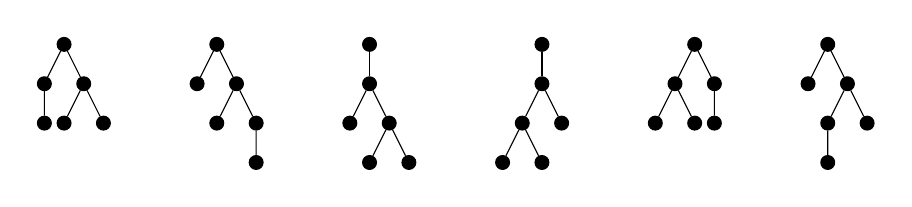
\begin{tikzpicture}[level distance=0.5cm,level/.style={sibling distance=0.5cm}]

    \matrix[column sep=1cm]
    {
      \node[vertex] {}
        child {node[vertex] {}
          child {node[vertex] {}}
        }
        child {node[vertex] {}
          child {node[vertex] {}}
          child {node[vertex] {}}
        };
    &
      \node[vertex] {}
        child {node[vertex] {}}
        child {node[vertex] {}
          child {node[vertex] {}}
          child {node[vertex] {}
            child {node[vertex] {}}
          }
        };
    &
      \node[vertex] {}
        child {node[vertex] {}
          child {node[vertex] {}}
          child {node[vertex] {}
            child {node[vertex] {}}
            child {node[vertex] {}}
          }
        };
    &
      \node[vertex] {}
        child {node[vertex] {}
          child {node[vertex] {}
            child {node[vertex] {}}
            child {node[vertex] {}}
          }
          child {node[vertex] {}}
        };
    &
      \node[vertex] {}
        child {node[vertex] {}
          child {node[vertex] {}}
            child {node[vertex] {}}
          }
        child {node[vertex] {}
          child {node[vertex] {}}
        };
    &
      \node[vertex] {}
        child {node[vertex] {}}
        child {node[vertex] {}
          child {node[vertex] {}
            child {node[vertex] {}}
          }
          child {node[vertex] {}}
        };
    \\
    };

  \end{tikzpicture}

\end{figure}

\subsection{Ambiguous Grammars}

In general an ambiguous grammar is a grammar where there is a string that can have more than one \todo{Define leftmost derivation} leftmost derivation. This also applies to hypergraph grammars.

The Hickey-Cohen generation algorithm requires the input grammar to be unambiguous in order to \emph{uniformly} generate terminal graphs. However, if the input grammar is ambiguous then the algorithm will generate graphs where each \emph{lefthand derivation} is uniformly distributed. Therefore if a terminal graph in the grammar has two lefthand derivations then this terminal graph has double the probability of being generated and therefore the generation is no longer uniform.

\todo{Example}

Unfortunately it is undecidable to know whether a grammar is ambiguous and impossible to convert an ambiguous grammar to an unambigous grammar. However as long as the user is aware that using an ambiguous grammar will not produce uniform results then there should be no problem.

\subsection{Cyclic Grammars}

A cyclic grammar is a grammar where a non-terminal can derive exactly itself. This can be directly ($A \Rightarrow A$) or indirectly ($A \Rightarrow B \Rightarrow A$). If a grammar contains epsilon productions, it may be cycling also in the case where $A \to AB$ and $B \to \epsilon$

The Hickey-Cohen approach is invalid on a cyclic grammar because the number of deriving strings from a cyclic non-terminal is infinite. We can observe this by expanding the generating function for a a simple grammar $A \to B | a$ and $B \to A$. The generating function becomes $g_A(t) = g_B(t) + \delta_0(t-1) = g_A(t) + \delta_0(t-1)$ which is recursive and cannot be computed.

In order to test if a grammar is cyclic, firstly the grammar must be transformed to an $\epsilon$-free grammar. This means there is no derivations to $\epsilon$ or there is exactly one $\epsilon$-production $S \to \epsilon$ and $S$ does not appear on the rightside of any production. In string grammars $\epsilon$ means the empty string, in hypergraph grammars $\epsilon$ means a graph containing just external nodes.

I will modify the algorithm to work with hypergraph grammars.

\begin{itemize}
\item Given a hypergraph grammar $G = \langle N, T, P, S \rangle$
\item Construct $N_\epsilon = \left\{A | A \in N \textrm{ and } A \Rightarrow^{+} \epsilon \right\}$. This is the set of non-terminals which possibly derive to $\epsilon$.

Define a predicate `$a$ produces $\epsilon$' which yields true if a non-terminal $a$ produces $\epsilon$. It is defined by the following: $A \to \langle R, ext \rangle$ is in $P$ where $R = \langle V, E, att, lbl\rangle$, $V = ext$ and $E = \{\}$. This means the production replaces a hyperedge with the empty graph.
\begin{enumerate}
\item Let $V_0 = \{A| \textrm{if $A \in N$ produces $\epsilon$}\}$ and set $i = 1$
\item Let $V_i = \left\{A| \textrm{if } A \to X_1X_2\dots X_n \textrm{ where } X_k \in V_{i-1}\right\} \cup V_{i-1}$
\item If $V_i \neq V_{i-1}$ set $i=i+1$ and repeat step 2. Otherwise let $N_\epsilon = V_i$
\end{enumerate}
Since $V_i \subseteq N$ then this procedure will terminate after a finite number of steps.
\item Let $P'$ be the set of productions constructed by the following
\begin{enumerate}
\item If $A \to \langle R, ext \rangle$ is in $P$, $k \geq 0$ and each $B_i$ is in $N_\epsilon$ but no symbols in any $a_j$ are in $N_\epsilon$, then add to $P'$ all productions in the form of
\[
A \to a_0 X_1 a_1 X_2 a_2 \dots X_k a_k
\]
Where $X_i$ is either $B_i$ or $\epsilon$, without adding $A \to \epsilon$.
\item If $S$ is in $N_\epsilon$, add to $P'$ the productions
\[S' \to \epsilon|S\]
Where $S'$ is a new symbol, and let $N' = N \cup \{S'\}$. Otherwise let $N' = N$ and $S' = S$
\end{enumerate}
\item Let $G' = \langle N', \Sigma, P', S' \rangle$
\end{itemize}

\paragraph{}

For example, given the grammar with the following productions in $P$:
\begin{align*}
A &\to AaBbCc | \epsilon \\
B &\to AB | \epsilon \\
C &\to c | d
\end{align*}
Then $V_\epsilon = \{A, B\}$ and the productions added to $P'$ would be:
\begin{align*}
A &\to AaBbCc | aBbCc | AabCc | abCc \\
B &\to AB | A | B \\
C &\to c | d \\
\end{align*}
This is an equivalent grammar without any $\epsilon$ productions.

\todo{Algorithm 2.10 The Theory of Parsin, Translation and Compiling Volume 1}

% The Hickey-Cohen approach also has a problem with the grammar $A \Rightarrow AB$, the counting function is: 
% \begin{align}
% g_A(t) &= (g_A * g_B)(t)
% &= \sum_{k=0}^{t} g_A(k) * g_B(t-k)
% \end{align}

% As we can see, this is a recursive function when $k=t$. This will cause an infinite loop when implemented in code so it would be good to remove this case. If it is known that $g_N(0)=0$ then we can update the function 

\section{Design}

\subsection{Language}
  The language and platform that the program runs on needs to be considered. Since the author's main operating system is Apple Mac OSX and the university's main operating systems are Microsoft Windows and Linux then it is required that the language chosen will run on these three operating systems.

  \subsubsection{The Java Virtual Machine}
    The first obvious choice is the \emph{Java} system by Sun Microsystems in 1991 and now Oracle Corporation since 2009. Java is a cross-platform runtime environment which runs on over 1.1 billion desktop computers worldwide\footnote{http://www.java.com/en/about/}.

    Java achieves cross-platform by using a virtual machine called Java Virtual Machine or JVM. Java programs are written and compiled into Java bytecode which can be subsequently run on any JVM implementation. JVM implementations exist on all major operating systems and Mac OSX bundles a JVM with installation.

    Other than the excellent cross-platform support, the JVM has more advantages. The Java runtime has great built-in graphical user interface library called Swing which can be used to create interfaces that will work on each operating system. This is good for the program created for this project since it provides a unified interface.

    The maturity and widespread use of the JVM leads to many highly used third-party libraries. Many different graph libraries exist that will be considered later.

    The fact that the Java system is used by billions of devides ensures that support for the JVM will continue into the future. This is important for users such as myself that wish to devote time into building an application and want that application to continue to work in many years to come.

    The speed of the JVM has increased over the years due to many optimisation techniques such as Just-in-time compilation and HotSpot which analyses a programs performance and optimised frequently excecuted code paths. Another technique is garbage collection which attempts to reclaim memory that is no longer in use by the program.

    Programs that involve computationally expensive procedures---such as this project---it is beneficial that the program can distribute computations across multiple cores of a computer. This is only possible if the runtime environment supports concurrency. Java has been designed to support concurrency by having built-in constructs for threading. 

    \paragraph{}

    \textbf{Java} is also the name of the main programming language that is supported by the Java runtime. It has a similar style to the popular languages C/C++ but currently lacks in certain modern language features to aid development. The Java Virtual Machine runs Java bytecode which means third-party languages are being developed for it such as Groovy, Clojure and Kotlin. In fact, any language can be compiled to Java bytecode as long as it can be internally expressed as Java bytecode. Some examples include JavaScript as Rhino, Python as Jython and Ruby as JRuby.

    \textbf{Scala} is such a language that has been developed to run on the JVM. Scala first appeared in 2003 and has been a popular choice over Java for a number of reasons.
    Scala has all the positive aspects of running on the JVM as well as improved syntax, type inference, pattern matching, operator overloading. These features help to improve expressiveness.

    Scala also has many functional characteristics such as anonymous functions and closures as first-class citizens, immutable data structures, map/filter/fold methods. These features are a huge benefit over Java especially when implementing mathematical concepts as this project does. For example using higher-order functions makes it easier to describe exactly what needs to be computed while abstracting implementation details away.

    On the other hand, Scala is a relatively new language compared to Java and as such it is slightly `rough around the edges'. The Integrated Development Environment support is not as good as Java and occasionally compile errors are slightly confusing but this is a steady process and these things are improving over time. There is also new syntax to learn which is a potential problem for users.

    In conclusion, using Scala provides improved programming constructs while still employing the benefits of the JVM.

\subsection{External Libraries}
  A code library is a collection of code that one or more people have brought together in a way that other people can use. The use of external libraries in an application can aid development because this code is generally proved to work by use of automated tests. This can cut time of development since it is a section of code that the developer does not need to worry about.

  For this project, it would be beneficial to use a graph library where many graph modification operations are already implemented.

  \subsubsection{Java Universal Network/Graph Framework}
  Java Universal Network/Graph Framework or \emph{JUNG} is a Java library that provides functions for the modeling, analysis and visualisation of graphs and networks. The JUNG architecture supports a variety of graph representations such as directed/undirected, multi-graphs and importantly hypergraphs.

  JUNG provides a highly extensible visualisation framework which enables a developer to show the structure of a graph in a range of different ways with custom layouts, filtering mechanisms and styles.

  The library was designed by a software engineer working at Google and a researcher at Microsoft. It is also partially funded by the National Science Foundation which shows the library is high Unfortunately the last update was in 2011 but it is opensource and available under the Berkeley Software Distribution (BSD) license so this means anybody is free to contribute to it.

  Internally, JUNG uses interfaces to refer to different types of graph. In programming an interface defines what operations the object must have but the implementation can choose how to do it. JUNG supports hypergraph interfaces but only has a concrete implementation for `set hypergraphs' which do not order the tentacles. Fortunately JUNG is designed to be extensible and implementing an sequential hypergraph is trivial. Furthermore, there is no built in support for visualising hypergraphs but again, this can be done fairly easily.

\subsection{File Representation}

    
\bibliography{references}{}
\bibliographystyle{plain}

\end{document}
